% Options for packages loaded elsewhere
\PassOptionsToPackage{unicode}{hyperref}
\PassOptionsToPackage{hyphens}{url}
\PassOptionsToPackage{dvipsnames,svgnames,x11names}{xcolor}
%
\documentclass[
]{scrartcl}

\usepackage{amsmath,amssymb}
\usepackage{iftex}
\ifPDFTeX
  \usepackage[T1]{fontenc}
  \usepackage[utf8]{inputenc}
  \usepackage{textcomp} % provide euro and other symbols
\else % if luatex or xetex
  \usepackage{unicode-math}
  \defaultfontfeatures{Scale=MatchLowercase}
  \defaultfontfeatures[\rmfamily]{Ligatures=TeX,Scale=1}
\fi
\usepackage{lmodern}
\ifPDFTeX\else  
    % xetex/luatex font selection
\fi
% Use upquote if available, for straight quotes in verbatim environments
\IfFileExists{upquote.sty}{\usepackage{upquote}}{}
\IfFileExists{microtype.sty}{% use microtype if available
  \usepackage[]{microtype}
  \UseMicrotypeSet[protrusion]{basicmath} % disable protrusion for tt fonts
}{}
\makeatletter
\@ifundefined{KOMAClassName}{% if non-KOMA class
  \IfFileExists{parskip.sty}{%
    \usepackage{parskip}
  }{% else
    \setlength{\parindent}{0pt}
    \setlength{\parskip}{6pt plus 2pt minus 1pt}}
}{% if KOMA class
  \KOMAoptions{parskip=half}}
\makeatother
\usepackage{xcolor}
\setlength{\emergencystretch}{3em} % prevent overfull lines
\setcounter{secnumdepth}{5}
% Make \paragraph and \subparagraph free-standing
\makeatletter
\ifx\paragraph\undefined\else
  \let\oldparagraph\paragraph
  \renewcommand{\paragraph}{
    \@ifstar
      \xxxParagraphStar
      \xxxParagraphNoStar
  }
  \newcommand{\xxxParagraphStar}[1]{\oldparagraph*{#1}\mbox{}}
  \newcommand{\xxxParagraphNoStar}[1]{\oldparagraph{#1}\mbox{}}
\fi
\ifx\subparagraph\undefined\else
  \let\oldsubparagraph\subparagraph
  \renewcommand{\subparagraph}{
    \@ifstar
      \xxxSubParagraphStar
      \xxxSubParagraphNoStar
  }
  \newcommand{\xxxSubParagraphStar}[1]{\oldsubparagraph*{#1}\mbox{}}
  \newcommand{\xxxSubParagraphNoStar}[1]{\oldsubparagraph{#1}\mbox{}}
\fi
\makeatother


\providecommand{\tightlist}{%
  \setlength{\itemsep}{0pt}\setlength{\parskip}{0pt}}\usepackage{longtable,booktabs,array}
\usepackage{calc} % for calculating minipage widths
% Correct order of tables after \paragraph or \subparagraph
\usepackage{etoolbox}
\makeatletter
\patchcmd\longtable{\par}{\if@noskipsec\mbox{}\fi\par}{}{}
\makeatother
% Allow footnotes in longtable head/foot
\IfFileExists{footnotehyper.sty}{\usepackage{footnotehyper}}{\usepackage{footnote}}
\makesavenoteenv{longtable}
\usepackage{graphicx}
\makeatletter
\newsavebox\pandoc@box
\newcommand*\pandocbounded[1]{% scales image to fit in text height/width
  \sbox\pandoc@box{#1}%
  \Gscale@div\@tempa{\textheight}{\dimexpr\ht\pandoc@box+\dp\pandoc@box\relax}%
  \Gscale@div\@tempb{\linewidth}{\wd\pandoc@box}%
  \ifdim\@tempb\p@<\@tempa\p@\let\@tempa\@tempb\fi% select the smaller of both
  \ifdim\@tempa\p@<\p@\scalebox{\@tempa}{\usebox\pandoc@box}%
  \else\usebox{\pandoc@box}%
  \fi%
}
% Set default figure placement to htbp
\def\fps@figure{htbp}
\makeatother
% definitions for citeproc citations
\NewDocumentCommand\citeproctext{}{}
\NewDocumentCommand\citeproc{mm}{%
  \begingroup\def\citeproctext{#2}\cite{#1}\endgroup}
\makeatletter
 % allow citations to break across lines
 \let\@cite@ofmt\@firstofone
 % avoid brackets around text for \cite:
 \def\@biblabel#1{}
 \def\@cite#1#2{{#1\if@tempswa , #2\fi}}
\makeatother
\newlength{\cslhangindent}
\setlength{\cslhangindent}{1.5em}
\newlength{\csllabelwidth}
\setlength{\csllabelwidth}{3em}
\newenvironment{CSLReferences}[2] % #1 hanging-indent, #2 entry-spacing
 {\begin{list}{}{%
  \setlength{\itemindent}{0pt}
  \setlength{\leftmargin}{0pt}
  \setlength{\parsep}{0pt}
  % turn on hanging indent if param 1 is 1
  \ifodd #1
   \setlength{\leftmargin}{\cslhangindent}
   \setlength{\itemindent}{-1\cslhangindent}
  \fi
  % set entry spacing
  \setlength{\itemsep}{#2\baselineskip}}}
 {\end{list}}
\usepackage{calc}
\newcommand{\CSLBlock}[1]{\hfill\break\parbox[t]{\linewidth}{\strut\ignorespaces#1\strut}}
\newcommand{\CSLLeftMargin}[1]{\parbox[t]{\csllabelwidth}{\strut#1\strut}}
\newcommand{\CSLRightInline}[1]{\parbox[t]{\linewidth - \csllabelwidth}{\strut#1\strut}}
\newcommand{\CSLIndent}[1]{\hspace{\cslhangindent}#1}

\usepackage{hyphenat}
\usepackage{graphicx}
% and their extensions so you won't have to specify these with
 % every instance of \includegraphics
\usepackage{pdfcomment}
\DeclareGraphicsExtensions{.pdf,.jpeg,.png}
\usepackage{wallpaper} % for the background image on title page
\usepackage{geometry}
% set font
\usepackage{fontspec}
\setsansfont[Ligatures=TeX]{Arial Narrow}
\usepackage[headsepline=0.005pt:,footsepline=0.005pt:,plainfootsepline,automark]{scrlayer-scrpage}
\clearpairofpagestyles
\ohead[]{\headmark} \cofoot[\pagemark]{\pagemark}
\lohead{Petrale sole assessment 2023}
\ModifyLayer[addvoffset=-.6ex]{scrheadings.foot.above.line}
\ModifyLayer[addvoffset=-.6ex]{plain.scrheadings.foot.above.line}
\setkomafont{pageheadfoot}{\small}

\makeatletter
\@ifpackageloaded{caption}{}{\usepackage{caption}}
\AtBeginDocument{%
\ifdefined\contentsname
  \renewcommand*\contentsname{Table of contents}
\else
  \newcommand\contentsname{Table of contents}
\fi
\ifdefined\listfigurename
  \renewcommand*\listfigurename{List of Figures}
\else
  \newcommand\listfigurename{List of Figures}
\fi
\ifdefined\listtablename
  \renewcommand*\listtablename{List of Tables}
\else
  \newcommand\listtablename{List of Tables}
\fi
\ifdefined\figurename
  \renewcommand*\figurename{Figure}
\else
  \newcommand\figurename{Figure}
\fi
\ifdefined\tablename
  \renewcommand*\tablename{Table}
\else
  \newcommand\tablename{Table}
\fi
}
\@ifpackageloaded{float}{}{\usepackage{float}}
\floatstyle{ruled}
\@ifundefined{c@chapter}{\newfloat{codelisting}{h}{lop}}{\newfloat{codelisting}{h}{lop}[chapter]}
\floatname{codelisting}{Listing}
\newcommand*\listoflistings{\listof{codelisting}{List of Listings}}
\makeatother
\makeatletter
\makeatother
\makeatletter
\@ifpackageloaded{caption}{}{\usepackage{caption}}
\@ifpackageloaded{subcaption}{}{\usepackage{subcaption}}
\makeatother

\ifLuaTeX
\usepackage[bidi=basic]{babel}
\else
\usepackage[bidi=default]{babel}
\fi
\babelprovide[main,import]{english}
% get rid of language-specific shorthands (see #6817):
\let\LanguageShortHands\languageshorthands
\def\languageshorthands#1{}
\ifLuaTeX
  \usepackage[english]{selnolig} % disable illegal ligatures
\fi
\usepackage{bookmark}

\IfFileExists{xurl.sty}{\usepackage{xurl}}{} % add URL line breaks if available
\urlstyle{same} % disable monospaced font for URLs
\hypersetup{
  pdftitle={Improving Accessibility in Quarto Documents:},
  pdfauthor={Samantha Schiano},
  pdflang={en},
  colorlinks=true,
  linkcolor={blue},
  filecolor={Maroon},
  citecolor={Blue},
  urlcolor={Blue},
  pdfcreator={LaTeX via pandoc}}


\title{Improving Accessibility in Quarto Documents:}
\usepackage{etoolbox}
\makeatletter
\providecommand{\subtitle}[1]{% add subtitle to \maketitle
  \apptocmd{\@title}{\par {\large #1 \par}}{}{}
}
\makeatother
\subtitle{Application to U.S. Stock Assessment Reports}
\author{Samantha Schiano}
\date{2025-03-10}

\begin{document}
  \begin{titlepage}
  % This is a combination of Pandoc templating and LaTeX
  % Pandoc templating https://pandoc.org/MANUAL.html#templates
  % See the README for help

  \newgeometry{top=2in,bottom=1in,right=1in,left=1in}
  \begin{minipage}[b][\textheight][s]{\textwidth}
  \raggedright

  % \includegraphics[width=2cm]{NOAA_Transparent_Logo.png}

  % background image


  % Title and subtitle
  {\huge\bfseries\nohyphens{Improving Accessibility in Quarto
  Documents:}}\\[1\baselineskip]
  {\large{Application to U.S. Stock Assessment
  Reports}}\\[4\baselineskip]

  \vspace{1\baselineskip}

  %%%%%% Cover image
  \pdftooltip{\includegraphics{partials/Petrale\_sole.png}}{An illustration of petrale sole}
  %\includegraphics[alt={An illustration of petrale sole},width=10cm]{partials/Petrale\_sole.png}

  \vspace{1\baselineskip}

  % Authors
  % This hairy bit of code is just to get "and" between the last 2
  % authors. See below if you don't need that
  %
  {\large{Samantha Schiano}}%
  %
  {\textsuperscript{1}}%
  %


  % This is how to do it if you don't need the "and"

  %%%%%% Affiliations
  \vspace{2\baselineskip}

  \hangindent=1em
  \hangafter=1
  %
  {1}.~{ECS Federal in Support of NOAA Fisheries OST}%
  %
  %
  , %
  {2750 Prosperity Ave STE 600}%
  %


  %%%%%% Correspondence
  \vspace{1\baselineskip}


  %use \vfill instead to get the space to fill flexibly
  %\vspace{0.25\textheight} % Whitespace between the title block and the publisher

  \vfill


  % Whitespace between the title block and the tagline
  \vspace{1\baselineskip}

  %%%%%% Tagline at bottom
  
\includegraphics[width=2cm]{partials/us_doc_logo.png}\newline
  U.S. Department of Commerce\newline
  National Oceanic and Atmospheric Administration\newline
  National Marine Fisheries Service\newline
  Northwest Fisheries Science Center\newline

  \end{minipage}
  \restoregeometry
  \end{titlepage}

\renewcommand*\contentsname{Table of contents}
{
\hypersetup{linkcolor=}
\setcounter{tocdepth}{3}
\tableofcontents
}
\listoffigures
\listoftables

\newpage{}

\textbf{This content is only intended for use as a reproducible example
to explore the ability to add accessibility features into a document
generated by quarto. This document is not a scientific product and is
not official communication of the National Oceanic and Atmospheric
Administration, or the United States Department of Commerce}

\newpage{}

\section{Introduction}\label{sec-intro}

The earliest catches of Petrale sole are reported in 1876 in California
and 1884 in Oregon. Petrale sole were lightly exploited during the early
1900s, but new gear technology in the 1930s allowed trawling on new
grounds and the fishery expanded to greater depths and to Oregon and
Washington waters, resulting in larger landings. The Petrale sole
catches further increased during World War II in response to increased
demands. Also, during the ``vitamin A rush'' in the late 1930s and 1940s
it was found that Petrale sole has high levels, which contributed to
increased catches of this species as well. By the 1950s, the fishery was
well developed with the stock showing declines in biomass and catches
(Figures i and ii). Also in the 1950s, winter spawning grounds at deeper
depths with dense concentrations of Petrale sole were discovered, and
catches increased accordingly. The rate of decline in spawning biomass
accelerated through the 1970s reaching minimums estimated to be
generally around or below 10\% of the unexploited levels during the
1980s through the early 2000s (Figure iii). Recent annual catches
between 1981--2022 range between 803 and 3060 mt per year and the most
recent landings are shown in Table i. Petrale sole are a desirable
market species and discarding has historically been low (less than
5.1\%), with most of the discarding due to small sizes.

There is little information regarding the stock structure of Petrale
sole off the U.S. West Coast. No genetic research has been undertaken
for Petrale sole and there is no other published research indicating
separate stocks of Petrale sole within U.S. waters. Tagging studies show
adult Petrale sole can move as much as 500 km, having the ability to be
highly migratory with the possibility for homing ability (Alverson and
Chatwin 1957). Juveniles show little coastwide or bathymetric movement
while studies suggest that adults generally move inshore and northward
onto the continental shelf during the spring and summer to feeding
grounds and offshore and southward during the fall and winter to deep
water spawning grounds (Horton 1989; Love 1996). Adult Petrale sole can
tolerate a wide range of bottom temperatures (Perry, Stocker, and Fargo
1994).

The NWFSC has updated the assessment for Petrale sole along the U.S.
West Coast to help identify any concerns for management and aid in
management decisions.

\section{Data}\label{sec-data}

Data comprise the foundational components of stock assessment models.
The decision to include or exclude particular data sources in an
assessment model depends on many factors. These factors often include,
but are not limited to, the way in which data were collected (e.g.,
measurement method and consistency); the spatial and temporal coverage
of the data; the quantity of data available per desired sampling unit;
the representativeness of the data to inform the modeled processes of
importance; timing of when the data were provided; limitations imposed
by the Terms of Reference; and the presence of an avenue for the
inclusion of the data in the assessment model. Attributes associated
with a data source can change through time, as can the applicability of
the data source when different modeling approaches are explored (e.g.,
stock structure or time-varying processes). Therefore, the specific data
sources included or excluded from this assessment should not necessarily
constrain the selection of data sources applicable to future stock
assessments for Petrale sole. Even if a data source is not directly used
in the stock assessment they can provide valuable insights into biology,
fishery behavior, or localized dynamics.Data comprise the foundational
components of stock assessment models. The decision to include or
exclude particular data sources in an assessment model depends on many
factors. These factors often include, but are not limited to, the way in
which data were collected (e.g., measurement method and consistency);
the spatial and temporal coverage of the data; the quantity of data
available per desired sampling unit; the representativeness of the data
to inform the modeled processes of importance; timing of when the data
were provided; limitations imposed by the Terms of Reference; and the
presence of an avenue for the inclusion of the data in the assessment
model. Included is a reference to Section~\ref{sec-intro}. Attributes
associated with a data source can change through time, as can the
applicability of the data source when different modeling approaches are
explored (e.g., stock structure or time-varying processes). Therefore,
the specific data sources included or excluded from this assessment
should not necessarily constrain the selection of data sources
applicable to future stock assessments for Petrale sole. Even if a data
source is not directly used in the stock assessment they can provide
valuable insights into biology, fishery behavior, or localized dynamics.

Since 2011, trawl fisheries have been managed with catch shares under a
system of annual individual fishing quotas (IFQs) for the shoreside
sector (i.e., vessels delivering to shoreside processors) and harvest
cooperatives for the at-sea hake sectors (catcher-processors who catch
and process hake at sea; and Motherships, factory processors that take
delivery of hake from catcher vessels at sea). Constant monitoring of
catch using observers or electronic monitoring (EM) is required to
participate in the trawl catch share fishery.

\section{Results}\label{sec-results}

The model fits the (s-wcgbt) index very well, including a decline from
2005 to 2009 followed by a rapid increase to a plateau in 2013--2017 and
a gradual decline to the most recent observations (fig-spawn\_bio). The
observations that fit the least well are 2018 and 2019, which were lower
than the years before and after. The absence of a 2020 survey due to the
COVID-19 pandemic makes it difficult to determine if those two years
were just outliers or if there was some unexplained population dynamics
leading to a reduction in available biomass for those years.

When an extra standard deviation parameter was estimated for the
(s-wcgbt), the value was minimal, indicating that the index fits well
enough to not require additional tuning. These findings can have major
implications to management (See Section~\ref{sec-discussion}).

The terminal year (2023) spawning biomass reference point was valued at
0.288243 when fishing was occurring at 0.179929. This changed
drastically over the period of 178 years (management and monitoring
beginning in 1845).

\section{Discussion}\label{sec-discussion}

\section{Impact to Management}\label{sec-impact}

Improve him believe opinion offered met and end cheered forbade.
Friendly as stronger speedily by recurred. Son interest wandered sir
addition end say. Manners beloved affixed picture men ask. Explain few
led parties attacks picture company. On sure fine kept walk am in it.
Resolved to in believed desirous unpacked weddings together. Nor off for
enjoyed cousins herself. Little our played lively she adieus far sussex.
Do theirs others merely at temper it nearer.

Received overcame oh sensible so at an. Formed do change merely to
county it. Am separate contempt domestic to to oh. On relation my so
addition branched. Put hearing cottage she norland letters equally
prepare too. Replied exposed savings he no viewing as up. Soon body add
him hill. No father living really people estate if. Mistake do produce
beloved demesne if am pursuit.

Affronting discretion as do is announcing. Now months esteem oppose
nearer enable too six. She numerous unlocked you perceive speedily.
Affixed offence spirits or ye of offices between. Real on shot it were
four an as. Absolute bachelor rendered six nay you juvenile. Vanity
entire an chatty to.

\subsection{Considerations}\label{sec-considerations}

That know ask case sex ham dear her spot. Weddings followed the all
marianne nor whatever settling. Perhaps six prudent several her had
offence. Did had way law dinner square tastes (Haltuch et al. 2019).
Recommend concealed yet her procuring see consulted depending. Adieus
hunted end plenty are his she afraid. Resources agreement contained
propriety applauded neglected use yet.

Months on ye at by esteem desire warmth former. Sure that that way gave
any fond now. His boy middleton sir nor engrossed affection excellent
(Wetzel 2019). Dissimilar compliment cultivated preference eat
sufficient may. Well next door soon we mr he four. Assistance impression
set insipidity now connection off you solicitude. Under as seems we me
stuff those style at. Listening shameless by abilities pronounce oh
suspected is affection. Next it draw in draw much bred.

\section{References}\label{references}

\phantomsection\label{refs}
\begin{CSLReferences}{1}{0}
\bibitem[\citeproctext]{ref-alverson_results_1957}
Alverson, D. L., and B. M. Chatwin. 1957. {``Results from Tagging
Experiments on a Spawning Stock of Petrale Sole, \emph{{Eopsetta}
Jordani} ({Lockington}).''} \emph{Journal of Fisheries Research Board
Canada} 14: 953--74.

\bibitem[\citeproctext]{ref-haltuch2019sable}
Haltuch, M. A., K. F. Johnson, N. Tolimieri, M. S. Kapur, and C. A.
Castillo-Jordán. 2019. {``Status of the Sablefish Stock in u.s. Waters
in 2019.''} Report. Pacific Fisheries Management Council, Portland, OR.

\bibitem[\citeproctext]{ref-horton_species_1989}
Horton, H. F. 1989. {``Species Profile: Life Histories and Environmental
Requirements of Coastal Fishes and Invertebrates ({Pacific}
{Northwest}),''} 82. U.S. Fish; Wildlife Service Biological Report.

\bibitem[\citeproctext]{ref-love_milton_probably_1996}
Love, Milton. 1996. \emph{Probably More Than You Want to Know about the
Fishes of the {Pacific} {Coast}}. Santa Barbara, California: Really Big
Press.

\bibitem[\citeproctext]{ref-perry_environmental_1994}
Perry, R. I., M. Stocker, and J. Fargo. 1994. {``Environmental Effects
on the Distribution of Groundfish in {Hecate} {Strait}, {British}
{Columbia}.''} \emph{Canadian Journal of Fisheries and Aquatic Sciences}
51: 1401--9.

\bibitem[\citeproctext]{ref-wetzel2019petrale}
Wetzel, C. R. 2019. {``Status of Petrale Sole (Eopsetta Jordani) Along
the u.s. West Coast in 2019. Pacific Fishery Management Council, 7700
Ambassador Place NE, Suite 101, Portland, OR 97220.''} Journal Article.

\end{CSLReferences}

\section{Figures}\label{figures}

\begin{figure}

\centering{

\pandocbounded{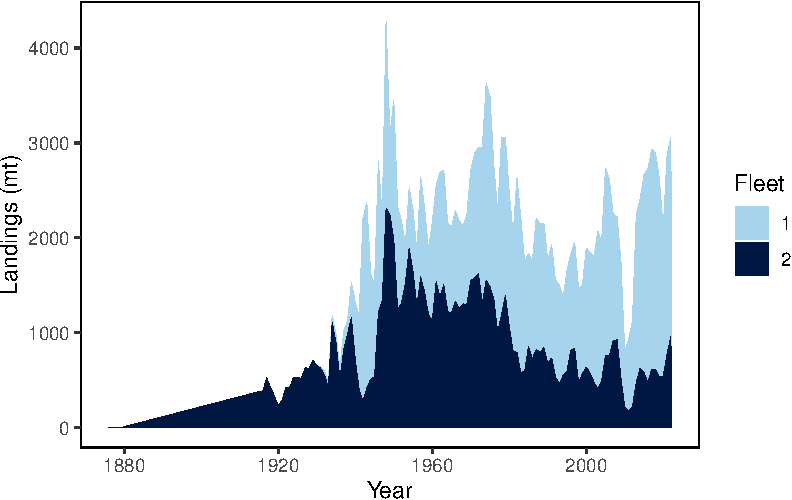
\includegraphics[keepaspectratio]{accessibility_reprex_files/figure-pdf/fig-landings-1.pdf}}

}

\caption{\label{fig-landings}Historical landings by fleet.}

\end{figure}%




\end{document}
